\documentclass{article}
\usepackage[dblblindworkshop,final]{neurips_2026}
\workshoptitle{Physical World AI: Geometry, Characteristics, and Multimodal Sensing}
\usepackage[T1]{fontenc}
\usepackage[utf8]{inputenc}
\usepackage{amsmath,amssymb}
\usepackage{graphicx,booktabs}
\usepackage{microtype}
\usepackage{url}
\usepackage[hidelinks]{hyperref}
\hypersetup{pdftitle={Decision-Level Auditing of Latent Robot World Models},
  pdfauthor={Anikait Rana, Siddhant Rana, Aditya Rao Udupi}}

\title{Decision-Level Auditing\\of Latent Robot World Models}
\author{Anikait Rana \qquad
Siddhant Rana \qquad Aditya Rao Udupi\\
Independent Researchers}

\begin{document}
\maketitle

\begin{abstract}
World models are often evaluated by prediction accuracy, but planning depends
on the actions their predictions select. We test whether correcting terminal
predictions selects physically better actions. On Push-T and Wall, we replace
predicted terminal representations with encodings of simulator endpoints reached
after executing the same 300 candidate action sequences. Actions, the goal,
encoder, and latent scoring objective remain fixed. Pooled across released
JEPA-WM and DINO-WM checkpoints, predicted scoring outperforms uniform choice on Push-T
distance utility and cumulative reward, and on Wall distance utility.
Endpoint correction changes 58.4\% and 55.9\% of valid choices, respectively,
but the original tests do not establish additional aggregate physical benefit.
Separately, a post-hoc state-distance selector chooses the realized endpoint
closest to the goal. Relative to realized-latent selection, it improves distance
utility by construction, reduces Push-T fixed-target cumulative reward, and
adds no observed Wall completions.
This hindsight diagnostic jointly bypasses the learned representation and
latent objective; it is not deployable and cannot isolate an encoder defect.
The audit distinguishes useful prediction-based selection, changed decisions,
and improved physical outcomes. Its findings concern fixed initial candidates,
not full CEM optimization or closed-loop control.
\end{abstract}

\section{Introduction}

A world model can predict imperfectly yet rank candidate actions usefully.
Conversely, an exact prediction can support a poor decision if the representation
and objective used to score it do not match the physical outcome of interest.
For example, correcting the predicted position of a robot may change which
action has the smallest visual-feature distance to a goal without improving
object placement. Prediction accuracy is therefore relevant to planning, but
does not by itself specify the value of a prediction correction.
Complete-controller success combines prediction, scoring, search, and candidate
support; it does not isolate that correction's contribution.

We ask a controlled question: \emph{if candidate actions, initial state, goal, encoder,
and scoring objective stay fixed, does replacing each predicted terminal
representation with the representation of what actually happened select a
physically better action?} An \emph{endpoint} is the simulator state reached
after executing the complete candidate action sequence. We encode its rendered
image and proprioceptive observation (the agent's own state) with the same
encoders used by the corresponding planner. Realized-endpoint scoring thus
removes terminal prediction error at this interface, but still judges actions
through the original latent goal objective. It is not a physical optimum.

We measure physical consequences separately: terminal distance to the supplied
goal state, cumulative official coverage reward on Push-T, and completion on
Wall. Push-T reward measures block overlap with the environment's fixed target,
not with the replay-generated goal used for terminal distance. A better value
on one outcome therefore need not imply improvement on another.

The audit separates four questions. Does predicted scoring contain useful
physical selection signal relative to uniform choice? How often does endpoint
replacement change the winner? Do those changes improve physical outcomes?
Finally, how much terminal-distance headroom remains when selection bypasses
the learned representation and latent objective together? For the last question,
we add a post-hoc \emph{retrospective state-distance selector}, which chooses the
candidate with the smallest realized simulator-state distance to the goal.
It uses outcomes unavailable before execution and is not deployable. It is an
upper bound for distance utility on this fixed set, not for every task outcome.

We study Push-T manipulation and Wall navigation using frozen released JEPA-WM and
DINO-WM predictors \citep{terver2026drives,pmlr-v267-zhou25t}. Both use pretrained
DINOv2 visual features \citep{oquab2023dinov2}, although their preprocessing and
proprioceptive encodings differ. We freeze the initial 300 candidates sampled
before any cross-entropy-method (CEM) update. Updating their distribution would
confound endpoint replacement with candidate generation. The experiment audits
the score-to-decision interface on these initial sets; it does not evaluate
full CEM or closed-loop model-predictive control (MPC), which would replan after
new observations. Each candidate instead receives a complete open-loop replay.

Predicted scoring selects useful actions, and endpoint replacement changes
many decisions, but the original tests do not establish additional aggregate
physical improvement. The new state selector exposes substantial distance
headroom while reducing cumulative Push-T reward and adding no Wall completions
beyond realized-latent selection. The latter comparison is limited by sparse successful
candidates. These are findings of an audit, not the performance of a proposed
repair. Jointly changing representation and objective cannot identify a defect
in DINOv2 alone, or distinguish representation limitations from objective choice.

Our contribution is a controlled, candidate-matched evaluation of the physical
consequences of terminal prediction correction; a retrospective extension that
makes its remaining objective dependence explicit; and a locally verified
candidate-level recomputation package prepared for release, with trajectory-
and case-level uncertainty. The
scope is intentionally narrower than a claim about which world model or
planning algorithm is best.

\section{Related work}

\paragraph{Prediction accuracy and control utility.}
\citet{pmlr-v120-lambert20a} distinguish model-fitting objectives from downstream
control performance and study their mismatch in model-based reinforcement
learning. Goal-aware prediction \citep{pmlr-v119-nair20a} learns to emphasize
task-relevant aspects of future observations. These approaches motivate asking
which errors matter to decisions. Our intervention does not train a new loss:
it replaces terminal predictions inside an otherwise fixed scoring interface
and measures the actions that interface selects.

\paragraph{Value-aware and value-equivalent modeling.}
Value-aware model learning evaluates model discrepancies through value-function
classes rather than generic transition accuracy \citep{pmlr-v54-farahmand17a}.
Value equivalence requires models to agree on Bellman updates for specified
policy and function classes \citep{grimm2020value}; it is not generic equality
of action rankings. Our finite-candidate audit shares the principle that model
quality depends on use, but neither tests Bellman-update equivalence nor
establishes a value-equivalence theorem. It directly observes selected actions
and their simulator outcomes.

\paragraph{Latent world models and representation-space planning.}
Latent-dynamics methods support planning without predicting every pixel
\citep{pmlr-v97-hafner19a}. DINO-WM predicts pretrained patch features and plans
by comparing predicted terminal features with a goal \citep{pmlr-v267-zhou25t}.
\citet{terver2026drives} study architectural and planning factors in
joint-embedding predictive world models, including the imperfect relationship
between prediction validation losses and planning success. Predicting a future
embedding and measuring its distance to a goal are different uses of a latent
space, even when both employ squared error. We retain that goal-scoring
interface for the endpoint-correction comparison.

\paragraph{Decision-level evaluation and objective diagnosis.}
Success rates evaluate the complete interaction of a model, objective, search
procedure, and candidate support. Ranking and selected-action diagnostics can
separate some of these factors without constituting a new controller.
\citet{singh2026objective} probe position information and latent-goal geometry
in LeWorldModel on TwoRoom, and evaluate changed planning costs under CEM/MPC.
Our complementary question concerns fixed candidates: what changes when only
predicted endpoints are replaced, and what remains when a privileged native
criterion bypasses the latent interface? We neither isolate the objective
causally nor test an objective repair in closed-loop planning.

\section{Audit design}
\label{sec:method}

\subsection{The experiment before the equations}

For one initial state and goal, retain 300 candidate action sequences in a fixed
order. The world model predicts each terminal representation; the lowest
latent goal cost selects $a_{\mathrm{pred}}$. Execute exactly those same
sequences from the same simulator initial condition, encode their realized
endpoints, and apply exactly the same goal cost to select $a_{\mathrm{real}}$.
Evaluate both selected sequences using stored native simulator outcomes.
The post-hoc third selector, $a_{\mathrm{state}}$, chooses the smallest stored
terminal state distance, then is evaluated on \emph{both} physical outcomes.
It is not independently optimized for reward or success.

Figure~\ref{fig:overview} shows what each comparison changes. Within a model,
endpoint replacement holds its encoders, preprocessing, goal, objective,
candidate actions, and replay conditions fixed. The state-based comparison
changes the selection criterion as well as bypassing the encoders. All
comparisons reuse existing candidate outcomes; the camera-ready diagnostic
requires no new training, prediction, or simulation.

\begin{figure}[t]
\centering
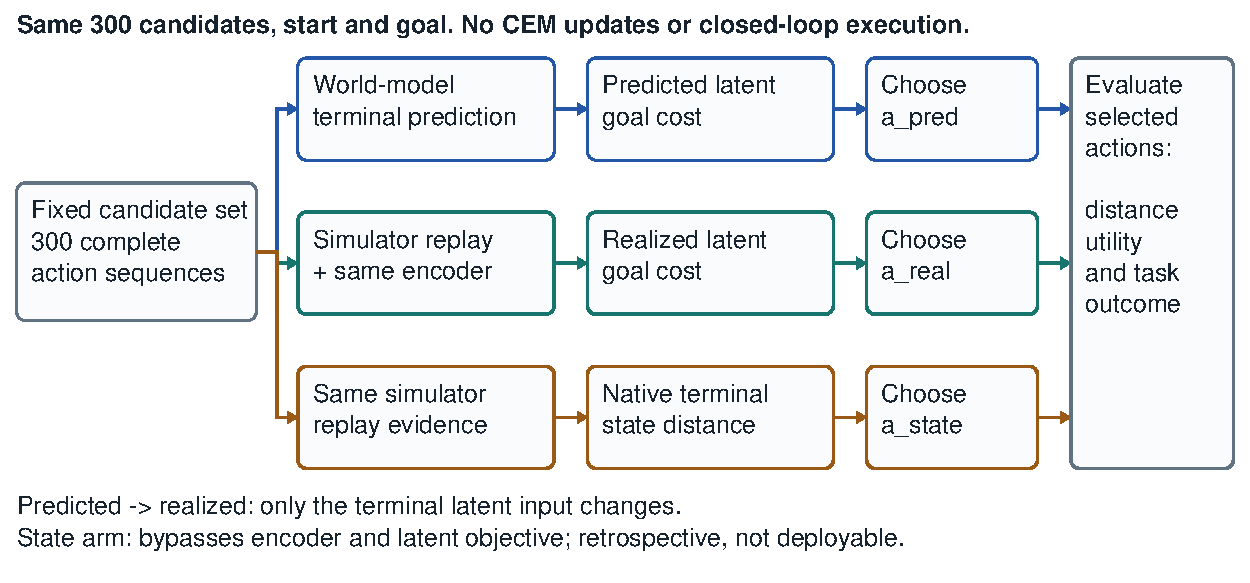
\includegraphics[width=\linewidth]{audit_overview.pdf}
\caption{Three selectors on the same ordered set of 300 action sequences.
Endpoint correction replaces predicted representations with encodings of
realized endpoints under the same latent objective. The retrospective state
selector additionally bypasses that representation and objective. All selected
actions are evaluated on the same native outcomes; only the first selector
uses information available before candidate execution.}
\label{fig:overview}
\end{figure}

\subsection{Costs, selectors, and physical outcomes}

Let $a_i$, $i\in\{1,\ldots,300\}$, denote a complete candidate sequence.
For the fixed initial observation, the world model produces a terminal latent
$\hat z_i$; encoding the realized terminal observation produces $z_i$.
The goal encoding is $z_g$. Each latent has visual and proprioceptive
components, denoted by superscripts $v$ and $p$. The released terminal cost is
\begin{equation}
 \begin{aligned}
 C(z,z_g)&=\frac{\|z^v-z_g^v\|_2^2}{d_v}
           +0.1\frac{\|z^p-z_g^p\|_2^2}{d_p},\\
 C_{\mathrm{pred}}(i)&=C(\hat z_i,z_g),\qquad
 C_{\mathrm{real}}(i)=C(z_i,z_g).
 \end{aligned}
 \label{eq:cost}
\end{equation}
where $d_v,d_p$ are the numbers of scalar coordinates in each component.
There is no sum of intermediate goal costs. The selectors are
\begin{equation}
 a_{\mathrm{pred}}=a_{\arg\min_i C_{\mathrm{pred}}(i)},\qquad
 a_{\mathrm{real}}=a_{\arg\min_i C_{\mathrm{real}}(i)},\qquad
 a_{\mathrm{state}}=a_{\arg\min_i D(s_i,s_g)},
 \label{eq:selectors}
\end{equation}
with realized terminal state $s_i$, goal state $s_g$, and the environment's
native distance $D$. The new state selector takes the first exact minimum
in stored candidate order. Existing selector-validation rules are preserved
(Appendix~\ref{app:protocol}); no exact minimum ties occur in the valid records.

Both reported outcomes are higher-is-better. Distance utility is
$U_{\mathrm{dist}}(a_i)=-D(s_i,s_g)$. The second outcome,
$R_{\mathrm{task}}(a_i)$, is cumulative official reward on Push-T and binary
completion on Wall. For example, endpoint correction has distance effect
\begin{equation}
 \Delta U_{\mathrm{dist}}^{\mathrm{real-pred}}
 =U_{\mathrm{dist}}(a_{\mathrm{real}})-U_{\mathrm{dist}}(a_{\mathrm{pred}}).
 \label{eq:effect}
\end{equation}
We also report state minus realized and state minus predicted, with the same
contrasts for $R_{\mathrm{task}}$. Distance gains for $a_{\mathrm{state}}$ are
nonnegative by construction; their magnitudes describe available fixed-set
headroom. No cumulative-reward guarantee follows on Push-T. On Wall, completion
thresholds that same distance, so the state selector also achieves the best
available binary completion in each candidate set. Uniform selection has
expected outcome equal to the mean over all 300 candidates, so its baseline
requires no additional random draw.

\section{Experiments and inference}

The experiments address four questions: \textbf{RQ1}, whether predicted scoring
improves physical outcomes over uniform choice; \textbf{RQ2}, how often endpoint
correction changes the selected sequence; \textbf{RQ3}, whether correction
improves aggregate physical outcomes; and \textbf{RQ4}, what remains under the
native terminal-state distance criterion. Switching describes decision sensitivity, not an
improvement criterion. The primary endpoint-correction contrast includes all retained
comparisons rather than conditioning inference on observed switches.

\paragraph{Shared setup.}
We audit released task-specific JEPA-WM and DINO-WM checkpoints. Each uses a
frozen DINOv2 ViT-S/14 visual backbone with 384-dimensional patch features and
$224\times224$ inputs. Proprioceptive encoders and image normalization remain
model-specific. Candidates are independent standard-normal samples in the
released normalized action coordinates, except the first candidate, fixed at the
normalized mean (stored index zero, mathematical index one). Each sequence
contains six model actions, each grouping five
two-dimensional physical actions: 30 simulator steps in total. Proposal seeds
are 1, 2, and 3. No CEM distribution update occurs. Appendix~\ref{app:config}
records transformations, checkpoints, and source bindings.
A record is one model's 300-candidate audit for one initial-state/goal instance
and proposal seed. Valid records pass the original artifact, complete-rollout,
finite-score/outcome, and selector checks; validity is not physical success.

\paragraph{Push-T.}
The agent pushes a T-shaped block toward a target configuration, using the
released Push-T implementation associated with these checkpoints; Push-T is
also used by \citet{chi2023diffusionpolicy}. We retain 20 validation trajectories,
five predetermined offsets per trajectory, three proposal seeds, and two
models: 600 scheduled model-level records. The goal is generated by replaying
the corresponding 30-step dataset action segment. The official native distance
is raw Euclidean distance over agent position, block position, raw block angle,
and agent velocity. It therefore mixes coordinates and units; it is neither
pure block-pose error nor task completion. $R_{\mathrm{task}}$ sums 30
official per-step rewards, each $\min\{\mathrm{coverage}/0.95,1\}$, where
coverage is the fraction of the environment's fixed target block area covered
by the current block. The target pose is $(256,256,\pi/4)$ and is not reassigned
to the segment's replay endpoint. Reward lies in $[0,30]$; it measures coverage
over time of that fixed target, whereas distance measures terminal agreement
with the segment-specific replay goal.

\paragraph{Analysis counts and missingness.}
There are 577 valid records and 281 offset--seed cells valid for both models
(562 records). The original analysis averages equally over the two models
inside each of 20 scheduled trajectory clusters, retaining a fixed denominator
of 15 offset--seed cells. Missing or unmatched cells contribute zero
\emph{contrast evidence}, not zero physical outcomes. This convention preserves
scheduled exposure but attenuates incomplete contributions. This same
convention applies to every selector contrast and model split. The reported
effect is an observed contrast contribution per scheduled cell, not a mean over
observed candidate sets alone. For example, if 14 of 15 scheduled cells are
matched and each has a model-averaged contrast of $+1$, that trajectory
contributes $14/15$, not $1$. The unmatched cell adds no contrast; neither
model is assigned a zero physical outcome.
The original study also included documented infrastructure recovery after a no-retry rule;
Appendix~\ref{app:protocol} reports the deviation, amendment, and an
original-completions-only sensitivity that fails the original support rule.

\paragraph{Wall.}
A point agent navigates around a wall through an opening toward a goal.
Thirty fixed initial-state/goal cases, three proposal seeds, and two models
give 180 scheduled records. One failed scientific record leaves 179 valid
records; inference uses the 29 cases with all six records present (174 records).
Native distance is terminal Euclidean position error, and completion means
distance strictly below 4.5. Successful candidates occur in only two complete
cases. Wall tests whether the correction finding is confined to Push-T's mixed-unit
state metric. It extends the audit to simpler state geometry, not to a strong
binary-success benchmark: sparse support restricts completion claims.

\paragraph{Dependence.}
Direct array checks confirm identical physical candidates and native outcomes
for all 281 retained cross-model Push-T pairs and all 89 available Wall pairs.
The state-selected action is therefore duplicated across paired model records,
not independent evidence. Equal model weighting compares it with two latent
selectors; uncertainty resamples whole trajectories or cases, never model rows
or candidates. Missing records receive no invented selector or physical outcome.

\paragraph{Original inference.}
The original inference uses 10,000 cluster-bootstrap draws, paired sign-flip
tests, and separate two-outcome Holm families for endpoint correction and
predicted-versus-uniform selection within each environment. The original
broad-recovery rule required support and stability checks, positive contrasts
on both outcomes under raw and bounded proposals, and the original interval
and Holm-test conditions (Appendix~\ref{app:protocol}). An isolated favorable
estimate could not establish that broad claim. We preserve those results unchanged.

\paragraph{Post-hoc diagnostic inference.}
The state-selector analysis is a new, post-hoc camera-ready diagnostic using
10,000 whole-cluster percentile-bootstrap draws and no new $p$-values. A common
resampling draw within each environment couples its three contrasts.
Consequently, its endpoint-correction point estimates reproduce the original
ones but its intervals can differ slightly due to the new shared random seeds.
Table~\ref{tab:ladder} reports these new intervals; original intervals and tests
remain separately labeled in Appendix~\ref{app:original}.

\section{Results}

\subsection{Useful selection signal does not imply useful endpoint correction}

Predicted scoring carried physical selection signal, but the original tests
did not establish an additional aggregate improvement from endpoint correction.
On Push-T, predicted-minus-uniform effects were $+48.70$ in distance utility
(95\% CI $[40.47,56.43]$) and $+0.761$ in cumulative reward
($[0.420,1.117]$), both passing their original Holm-adjusted tests.
The corresponding Wall distance effect was $+12.363$ ($[10.900,13.755]$);
its small completion effect was not established by the original test.
Thus a lack of added benefit from correction should not be confused with
an absence of useful signal in the original predicted scores.

For Push-T endpoint correction, the original distance estimate was $-5.299$
($[-9.635,-0.706]$, Holm-adjusted $p=0.0755$) and reward estimate $+0.042$
($[-0.176,0.240]$, adjusted $p=0.701$). The marginal distance interval excludes
zero, while the adjusted test does not meet the two-outcome decision threshold;
these are different inferential procedures, not interchangeable decisions.
Wall effects were $-0.254$ in distance utility ($[-0.909,0.364]$) and $+0.029$
in completion ($[0,0.080]$), each with adjusted $p=0.923$.
These results do not demonstrate equivalence between selectors.

\subsection{Endpoint replacement changes many choices}

The selectors often disagree even when aggregate physical improvement is not
established. Among all valid records, endpoint correction changes 337/577
Push-T choices (58.4\%) and 100/179 Wall choices (55.9\%).
Table~\ref{tab:disagreement} distinguishes these descriptive denominators from
the records retained for clustered physical comparisons. The state selector
usually differs from either latent selector. None of these switch rates by
itself indicates whether the new choice is physically preferable.
The frequent changes nevertheless show that endpoint correction materially
affects decisions: the absence of an established aggregate gain is not simply
an observation that the selected actions stayed the same.

\begin{table}[t]
\caption{Descriptive selector disagreements, counts and percentages.
``Analysis'' retains the original paired-cell or complete-case record set.
Records are not independent inferential units.}
\label{tab:disagreement}
\centering\small
\begin{tabular}{llrrr}
\toprule
Environment & Records & Predicted/realized & Realized/state & Predicted/state\\
\midrule
Push-T & All valid: 577 & 337 (58.4\%) & 525 (91.0\%) & 515 (89.3\%)\\
 & Analysis: 562 & 331 (58.9\%) & 511 (90.9\%) & 502 (89.3\%)\\
Wall & All valid: 179 & 100 (55.9\%) & 138 (77.1\%) & 144 (80.4\%)\\
 & Analysis: 174 & 100 (57.5\%) & 133 (76.4\%) & 139 (79.9\%)\\
\bottomrule
\end{tabular}
\end{table}

\subsection{State-distance headroom is substantial but objective-dependent}

Relative to realized-latent selection, the retrospective state selector improves
terminal distance while reducing Push-T cumulative reward and adding no observed
Wall completions.
Table~\ref{tab:ladder} and Figure~\ref{fig:ladder} report all three contrasts.
Push-T effects retain the scheduled-cell denominator described above.
Relative to realized-latent selection, Push-T distance utility increases by
$69.814$ ($[62.326,77.641]$), but cumulative reward decreases by $0.838$
($[-1.222,-0.460]$). Relative to predicted selection, the corresponding
effects are $+64.515$ and $-0.796$. The selector is a diagnostic, not a
proposed controller. It reveals that minimizing replay-goal whole-state
terminal distance does not optimize cumulative coverage of the environment's
fixed target. Both the target and temporal/objective definitions differ; the
reward decline does not isolate which difference caused the trade-off.

\begin{table}[t]
\caption{Post-hoc three-selector audit. Effects are first selector minus
second, with unadjusted 95\% whole-cluster percentile intervals. Higher is better for
both columns. Push-T reward is cumulative coverage; Wall reward is binary
completion. Distance units differ across environments. All intervals here
use the new common resampling draws, including realized minus predicted;
the unchanged original inference appears in Table~\ref{tab:original}.}
\label{tab:ladder}
\centering\small
\begin{tabular}{llrr}
\toprule
Environment & Contrast & $\Delta U_{\mathrm{dist}}$ [95\% CI] & $\Delta R_{\mathrm{task}}$ [95\% CI]\\
\midrule
Push-T & Realized $-$ predicted & $-5.299\ [-9.598,-0.720]$ & $+0.042\ [-0.167,0.242]$\\
 & State $-$ realized & $+69.814\ [62.326,77.641]$ & $-0.838\ [-1.222,-0.460]$\\
 & State $-$ predicted & $+64.515\ [58.162,71.121]$ & $-0.796\ [-1.192,-0.421]$\\
\addlinespace
Wall & Realized $-$ predicted & $-0.254\ [-0.915,0.363]$ & $+0.029\ [0,0.080]$\\
 & State $-$ realized & $+5.643\ [3.861,7.664]$ & $0\ [0,0]$\\
 & State $-$ predicted & $+5.390\ [3.902,7.090]$ & $+0.029\ [0,0.080]$\\
\bottomrule
\end{tabular}
\end{table}

On Wall, state-minus-realized distance utility is $+5.643$
($[3.861,7.664]$), but the completion contrast is exactly zero in all observed
complete cases. Its $[0,0]$ bootstrap interval reflects resampling those zero
contrasts, not an equivalence result or proof of zero population benefit.
Only five distinct successful physical candidate instances occur, across four
candidate sets in two cases. Predicted, realized, and state selection succeed
in 3, 8, and 8 of 174 repeated model records, respectively. Moreover, Wall
completion thresholds the same distance minimized by the state selector;
it is not independent corroboration of that distance objective. The state
selector must complete whenever any candidate can. Its equal completion count
therefore means that realized-latent selection already captured every available
completion in the retained successful sets. Wall's zero increment diagnoses
limited remaining completion support, not the distance/reward conflict seen on
Push-T.

\begin{figure}[t]
\centering
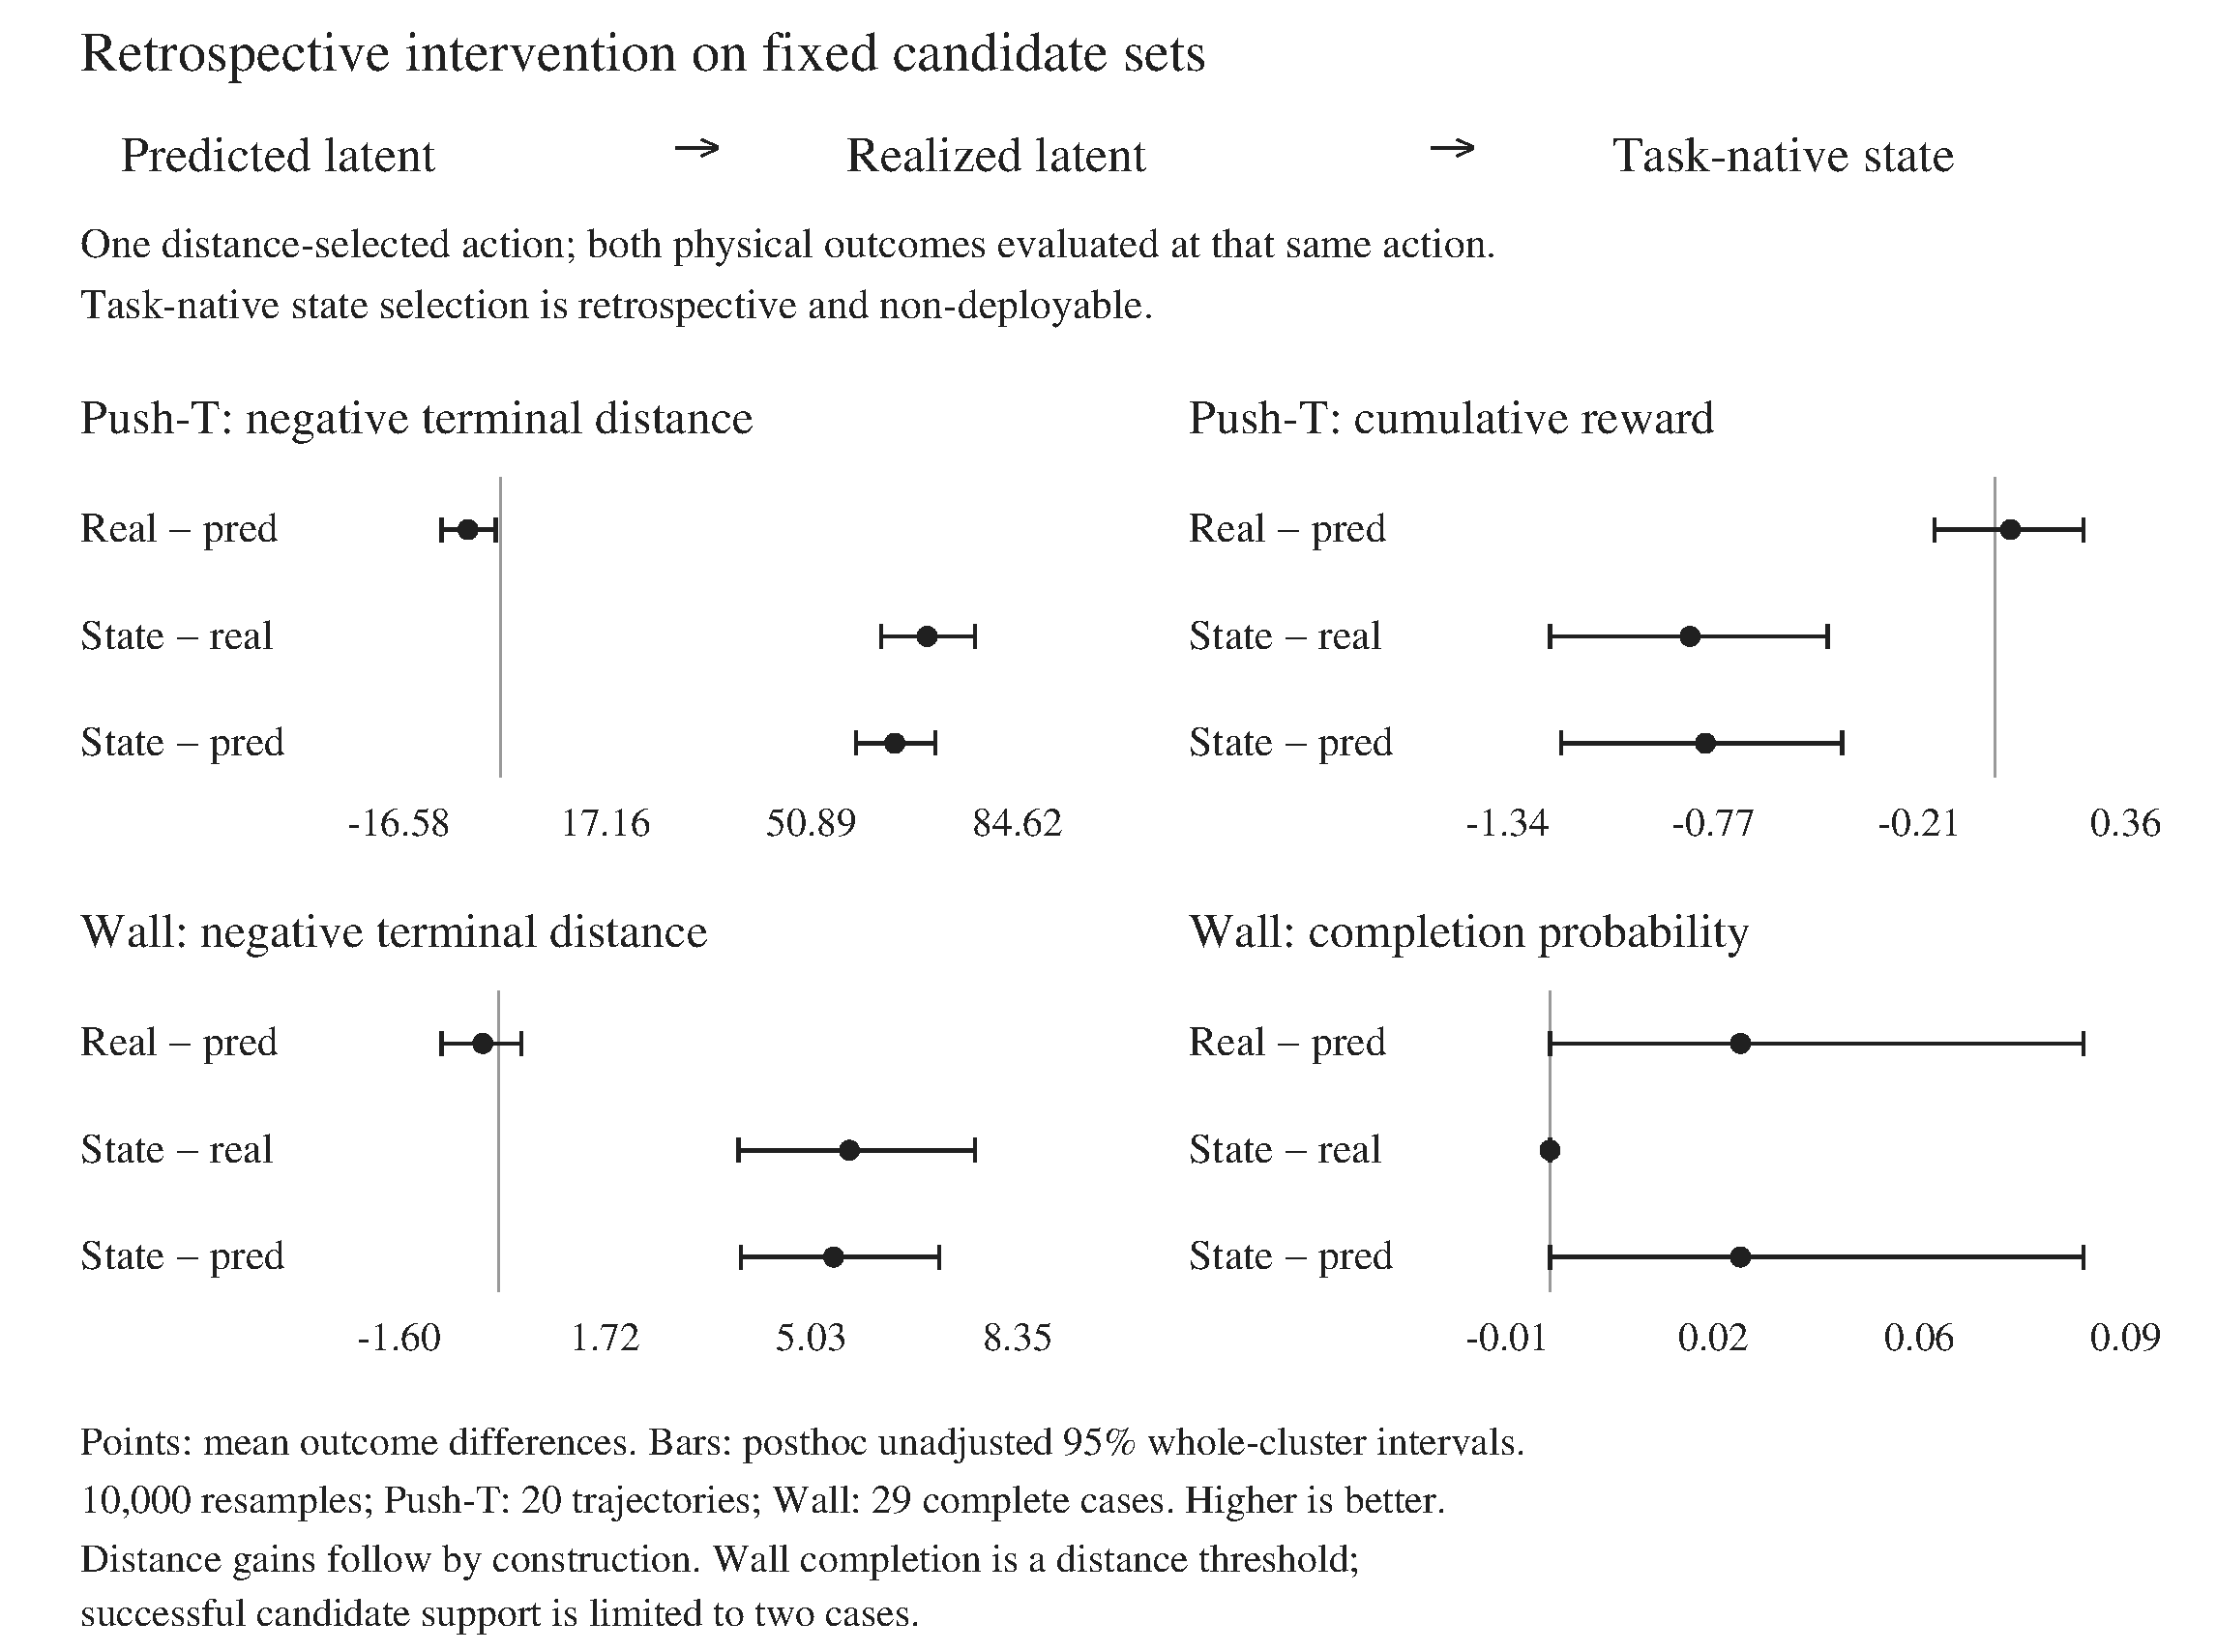
\includegraphics[width=\linewidth]{intervention_ladder.pdf}
\caption{Post-hoc physical effects along the intervention ladder, with
whole-trajectory or whole-case 95\% bootstrap intervals. The first step
corrects terminal predictions under a fixed latent objective. The second
jointly bypasses the representation and objective. Distance improvement in
the second step is definitional; relative to realized-latent selection, Push-T
reward declines and Wall completion is unchanged in the observed cases. These are diagnostic interventions,
not deployable stages of a planning algorithm.}
\label{fig:ladder}
\end{figure}

\subsection{Model and outcome decompositions qualify the aggregate story}

The pooled results conceal different endpoint-correction magnitudes, but both
models show the same adverse Push-T reward contrast for state selection.
Descriptively, Push-T realized-minus-predicted distance effects are $-9.330$
for JEPA-WM and $-1.268$ for DINO-WM; state-minus-realized reward effects are
$-0.861$ and $-0.815$. On Wall, endpoint-correction distance effects are
$-0.655$ and $+0.148$, while state-minus-realized distance effects are $+4.910$
and $+6.376$. Neither model adds observed completions in that second contrast.
Appendix~\ref{app:models} reports all descriptive model splits; there is no
preregistered model-interaction claim and no independent encoder comparison.

An earlier post-hoc Push-T component analysis further shows why aggregate
distance must not be read as block-placement quality. Realized-latent selection
improves block-position utility by $1.267$ and circular-angle utility by
$0.0325$ radians, while agent-position and velocity point estimates are adverse.
Velocity supplies the largest negative contribution to squared native distance.
The component results and their five-component adjustment are retained in
Appendix~\ref{app:sensitivity}; they do not identify a causal module.
An auxiliary near-tie score predicts selector changes but not established
physical harm. Its frozen Wall AUROC, $0.727$, is below the simple raw-margin
baseline's $0.735$, so it remains a secondary diagnostic rather than a central
contribution (Appendix~\ref{app:neartie}).

\section{Limitations and interpretation}

This audit establishes what the retained score-to-decision interfaces do on
fixed initial candidate sets. It does not establish full-CEM performance,
closed-loop benefit, learned correction quality, real-robot performance, or
generalization beyond the two simulation environments. Both predictor families
share DINOv2 weights, so they do not supply independent representation-family
evidence. Model-specific preprocessing also prevents treating their encoded
observations as identical.

Realized-latent selection corrects a terminal input to the objective, not the
objective itself. State selection jointly changes the representation and
criterion, and requires privileged realized outcomes. Its large distance gains
demonstrate available distance headroom, not that DINOv2 is defective, that an
objective-only change would recover it, or that a trainable method can attain
it. Push-T's mixed-unit distance and cumulative reward support different
conclusions, and its reward target is fixed independently of its replay goal. This prevents
attributing the observed reward trade-off purely to temporal aggregation or
to a learned representation defect. Wall's sparse and threshold-linked
completions prevent broad
success-rate claims.

The new selector, earlier component analysis, and Push-T near-tie analysis
are post-hoc. Whole-cluster resampling respects recorded dependence but cannot
remove selection bias from missing data. Push-T's recovery amendment and
fixed-denominator convention, and Wall's complete-case restriction, remain
substantive qualifications. Intervals describe cluster-resampling variation
in this selected collection; they do not establish population-wide performance
within either task. Marginal intervals are not equivalence intervals;
the original sign-flip tests additionally assume null sign symmetry.

\section{Conclusion}

Useful predicted scoring, sensitivity to prediction correction, and improved
physical decisions are distinct properties. Our fixed-candidate audit finds
the first two without an established additional aggregate benefit from
endpoint correction. Bypassing the latent interface reveals substantial
terminal-distance headroom, yet worsens cumulative Push-T reward and adds no
observed Wall completions beyond realized-latent selection. This objective-dependent result clarifies what the
audit measures without proposing a deployable fix or isolating an encoder
failure mechanism. The remaining distance headroom motivates investigating
the learned representation and latent goal objective as a joint planning
interface; the present intervention does not diagnose either component alone.

\clearpage
\bibliographystyle{plainnat}
\bibliography{references}

\clearpage
\appendix
\section{Notation and interpretation glossary}
\label{app:glossary}

\begin{table}[h]
\centering
\begin{tabular}{@{}p{0.27\linewidth}p{0.69\linewidth}@{}}
\toprule
Symbol or term & Meaning\\
\midrule
$a_i$ & Candidate $i$: a complete 30-step physical action sequence.\\
Endpoint $s_i$ & State after executing all actions in candidate $i$.\\
$z_i$, $\hat z_i$, $z_g$ & Encoded realized endpoint, predicted terminal latent, encoded goal.\\
$C_{\mathrm{pred}}$, $C_{\mathrm{real}}$ & The same latent goal cost evaluated on predicted or encoded realized endpoints.\\
$a_{\mathrm{pred}}$ & Candidate selected by predicted latent cost.\\
$a_{\mathrm{real}}$ & Candidate selected by realized-endpoint latent cost; retrospective, not a physical optimum.\\
$a_{\mathrm{state}}$ & Candidate minimizing realized native terminal distance; retrospective and non-deployable.\\
$D$, $U_{\mathrm{dist}}$ & Native distance and its negative, the higher-is-better distance utility.\\
$R_{\mathrm{task}}$ & Cumulative official Push-T coverage reward or Wall binary completion.\\
Record & One model, initial-state/goal instance, and proposal seed, with 300 candidates.\\
Paired cell & One Push-T trajectory offset and seed with valid records for both models.\\
Cluster & A scheduled Push-T trajectory or a complete Wall case; the resampling unit.\\
Initial candidates & Samples before any CEM distribution update; historically called an ``iteration-0 menu'' in code.\\
\bottomrule
\end{tabular}
\end{table}

\section{Original inference, unchanged}
\label{app:original}

Table~\ref{tab:original} retains the original pooled point estimates, percentile
intervals, and Holm-adjusted sign-flip values. Push-T uses all 20 scheduled
trajectory contrasts, 10,000 trajectory-bootstrap draws, and enumeration of
all $2^{20}$ sign assignments for its two-sided paired test. Wall uses 29
complete-case contrasts, 10,000 case-bootstrap draws (seed 20260911), and
100,000 random sign assignments with the $+1$ correction (seed 20260912).
Holm adjustment covers two outcomes separately for endpoint correction and
predicted-minus-uniform selection within each environment. Push-T's bounded
candidate sensitivity has its own originally declared two-outcome family.
The exact test requires sign symmetry of cluster contrasts under the null.
No new state-selector comparison has been added to those original families.

\begin{table}[h]
\caption{Unchanged original inference. Intervals are marginal 95\% cluster
bootstrap intervals; $p_H$ is the original within-family Holm-adjusted value.}
\label{tab:original}
\centering\small
\begingroup
\setlength{\tabcolsep}{3pt}
\begin{tabular}{lllrr}
\toprule
Environment & Contrast & Outcome & Effect [95\% CI] & $p_H$\\
\midrule
Push-T & Realized $-$ predicted & Distance utility & $-5.299\ [-9.635,-0.706]$ & .075539\\
 & & Reward & $+0.04183\ [-0.17569,0.24024]$ & .701128\\
 & Predicted $-$ uniform & Distance utility & $+48.702\ [40.473,56.434]$ & $7.6294\!\times\!10^{-6}$\\
 & & Reward & $+0.76099\ [0.42033,1.11714]$ & .00040245\\
Wall & Realized $-$ predicted & Distance utility & $-0.25365\ [-0.90933,0.36436]$ & .923091\\
 & & Completion & $+0.02874\ [0,0.08046]$ & .923091\\
 & Predicted $-$ uniform & Distance utility & $+12.36271\ [10.90015,13.75461]$ & $1.99998\!\times\!10^{-5}$\\
 & & Completion & $+0.01705\ [0,0.04544]$ & .501395\\
\bottomrule
\end{tabular}
\endgroup
\end{table}

The new diagnostic uses seeds 20261002 (Push-T) and 20261003 (Wall), with
10,000 whole-cluster draws shared by its three contrasts and both outcomes
within each environment. These intervals quantify the new post-hoc comparisons
and do not replace the original test decisions. Recomputing the original
results is a required preflight check before generating the new results.

\section{Model-specific descriptive comparisons}
\label{app:models}

Table~\ref{tab:models} uses the same retained cells, cluster definitions,
denominators, and common bootstrap draws as the pooled post-hoc analysis.
Each model estimate compares a latent selector with the same physical state
selector on matched sets. Repeated state-selected outcomes do not provide a
second physical experiment. All entries are descriptive; differences between
their confidence intervals are not model-interaction tests.

\begin{table}[h]
\caption{Post-hoc model-specific effects with 95\% cluster-bootstrap
intervals. ``Real'', ``pred'', and ``state'' refer to the three defined selectors.}
\label{tab:models}
\centering\small
\begin{tabular}{lllrr}
\toprule
Task & Model & Contrast & $\Delta U_{\mathrm{dist}}$ [95\% CI] & $\Delta R_{\mathrm{task}}$ [95\% CI]\\
\midrule
Push-T & JEPA-WM & Real $-$ pred & $-9.330\ [-14.394,-4.557]$ & $+.081\ [-.130,.280]$\\
 & & State $-$ real & $+67.623\ [59.887,76.057]$ & $-.861\ [-1.271,-.453]$\\
 & & State $-$ pred & $+58.293\ [50.879,65.943]$ & $-.780\ [-1.169,-.407]$\\
 & DINO-WM & Real $-$ pred & $-1.268\ [-7.898,6.272]$ & $+.003\ [-.241,.237]$\\
 & & State $-$ real & $+72.005\ [63.922,80.083]$ & $-.815\ [-1.179,-.462]$\\
 & & State $-$ pred & $+70.737\ [64.052,77.512]$ & $-.812\ [-1.229,-.420]$\\
\addlinespace
Wall & JEPA-WM & Real $-$ pred & $-.655\ [-1.649,.215]$ & $+.0345\ [0,.0920]$\\
 & & State $-$ real & $+4.910\ [3.327,6.785]$ & $0\ [0,0]$\\
 & & State $-$ pred & $+4.255\ [3.001,5.839]$ & $+.0345\ [0,.0920]$\\
 & DINO-WM & Real $-$ pred & $+.148\ [-.724,.923]$ & $+.0230\ [0,.0690]$\\
 & & State $-$ real & $+6.376\ [4.222,8.825]$ & $0\ [0,0]$\\
 & & State $-$ pred & $+6.524\ [4.551,8.761]$ & $+.0230\ [0,.0690]$\\
\bottomrule
\end{tabular}
\end{table}

\section{Sampling, missingness, and the recovery amendment}
\label{app:protocol}

\paragraph{Push-T selection and support.}
The manifest selects validation trajectory indices 0--20 except 7, for 20
trajectories, without consulting audit outcomes. For a trajectory of length
$L$, its five offsets are $\lfloor k(L-31)/4\rfloor$, $k=0,\ldots,4$.
Only recorded sequence lengths select the offsets. Expert block-state motion
labels a secondary phase proxy but does not select or exclude records.
Each offset is paired with proposal seeds 1, 2, and 3 and both models.
The resulting 100 distinct initial-state/goal segments produce 300 offset--seed
cells and 600 scheduled model records. The manifest's historical
\texttt{segment\_count=300} includes proposal seeds.

For an outcome $Y$ (either $U_{\mathrm{dist}}$ or $R_{\mathrm{task}}$), let
$\delta_{tcm}$ be a specified selector contrast for trajectory $t$, cell $c$,
and model $m$. The cell indicator $I_{tc}$ equals one only when both model
records are valid under the original rules. The pooled trajectory contrast is
\begin{equation}
 \bar\delta_t=\frac{1}{2}\sum_{m=1}^{2}
          \frac{1}{15}\sum_{c=1}^{15} I_{tc}\delta_{tcm},
 \qquad \widehat\Delta=\frac{1}{20}\sum_{t=1}^{20}\bar\delta_t.
 \label{eq:cluster}
\end{equation}
Missing-cell terms are defined as zero \emph{contrast contributions}; the
formula does not assign a physical outcome to a missing action. The two-model
mask and fixed 15-cell denominator are preserved for every new contrast and
model split. Observed-cell means would answer a different question.
The original support requirement is at least 540 matched model records and
at least 18 trajectories with 12 or more matched cells. The retained study
has 562 matched records and 19 such trajectories, so it meets that requirement;
all 20 scheduled trajectories still enter Eq.~\ref{eq:cluster}.
Support gates require coverage of the scheduled experiment, not a positive
physical effect or a guarantee of adequate power. The original broad-recovery
rule additionally required passed integrity and repeat-stability checks;
positive pooled means and lower 95\% bounds, with Holm-adjusted $p<.05$, for
both outcomes under raw and bounded candidates; positive model-specific lower
bounds for both outcomes in both candidate sets; and no conflicting pooled
signs. Failure of any condition blocked the broad claim. Sampling, outcomes,
aggregation, tests, and this rule were recorded in the original locked protocol;
recovery was a later amendment, and the auxiliary and new state-selector
analyses are separately labeled post-hoc.

\paragraph{Infrastructure recovery.}
The Push-T protocol was recorded as locked on August 30, 2026 and prohibited
retries. Its original 600-record attempt ledger ended with 420 completed and
180 failed records. A fatal CUDA error had contaminated the persistent worker,
causing later untouched records to receive the same infrastructure error.
The recovery amendment mechanically selected 169 failed records with that
exact error message for at most one attempt each, in isolated processes.
The remaining failure classes were not eligible. The amendment states that
eligibility was fixed before inspecting scientific outcomes, preserving
candidate specifications and analysis rules, but this remains a deviation
from the original no-retry rule. Original failures remain in the ledger;
recovery neither deletes them nor makes them original completions.
The no-retry rule restricted opportunities to change retained evidence through
selective repeated attempts; the amendment does not retroactively satisfy it.
The recovery-augmented analysis has
577 valid and 23 invalid records, with 15 valid records unmatched across models.
Removing every recovery-sourced artifact leaves 408 matched records and only
14 trajectories meeting the original eligibility threshold: the original-only
subset fails the original support requirement. Its distance and reward effects
are $-5.39$ ($[-9.32,-1.40]$) and $-0.019$ ($[-0.212,0.160]$), respectively.
These are exploratory sensitivity estimates, not a restored confirmatory
analysis or evidence that missingness is ignorable. The 15 observed trajectory
groups used by a separate diagnostic are not 15 eligible primary clusters.

Earlier protocol versions are not scientific inputs to this analysis: v1.2
failed its prescribed RGB/serialization integrity check, and v1.3 failed
before usable measurements because a replay-encoding helper lacked its
required model argument. The v1.4 source and evidence are separately bound;
no earlier-version result is reused. The retained protocol, amendment, and
ledgers make this history inspectable but do not constitute an independently
registered timestamp for the declared outcome-blind sequence.

\paragraph{Wall selection and missingness.}
Case seeds 2026091100--2026091129 generate the 30 initial-state/goal cases.
Engineering seeds 2026091001 and 2026091002 are excluded from the study.
The wall location is 32 and door location 30 in the underlying 65-pixel
environment. Each case contains seeds 1--3 and both models. One JEPA-WM
record, case \texttt{wall\_028}, seed 1, failed scientific validation and was
not retried. Its entire case is excluded from the complete-case physical
analysis. The remaining five valid records contribute only to all-valid
descriptions. Case contrasts average the six model--seed records equally;
the 29 case means are the inferential units. This restriction does not rule
out difficulty-dependent missingness.
The retained failure ledger labels this failure \texttt{scientific\_or\_child}
but supplies no error message, so its specific failed criterion is not
established by that ledger.

\paragraph{Integrity and ties.}
Original Push-T validity required finite production arrays, decomposition
residuals at most $10^{-8}$, and score reproduction within $2\times10^{-5}$
with zero relative tolerance. Re-encoding serialized observations at chunk
sizes eight and four had to preserve scores within that tolerance and the
latent minimum tie sets exactly. Original repeat and provenance checks also
applied. Execution completion alone therefore did not imply scientific
validity; a valid record still needed its partner for paired analysis.
The new preflight checks cover all 780 unique scheduled records: 756 valid
and 24 invalid across both environments. They verify candidate counts,
selectors, stored physical arrays, cross-model agreement, and the original
headline analysis before new computation. Push-T's original latent selectors
require a unique minimum under absolute tolerance $10^{-10}$ and relative
tolerance $10^{-8}$; otherwise that record is invalid. Wall's latent selectors
use the first exact minimum. The new state selector also uses the first exact
minimum. No exact minimum ties or duplicate physical sequences occur in the
retained valid candidate sets; synthetic tests cover deterministic tie
handling. Cross-model identity is established by arrays, not assumed from
shared random-seed labels.

\section{Model and environment configuration}
\label{app:config}

\paragraph{Visual encoding.}
Both models in both tasks load \texttt{dinov2\_vits14} from
\texttt{dinov2\_vits14\_pretrain.pth}: a ViT-S/14 with 384-dimensional patch
features. Raw RGB is divided by 255 and resized to $224\times224$ using
bilinear interpolation with \texttt{align\_corners=False}. The audit loaders
fix spatial scale and aspect-ratio augmentation ranges to $(1,1)$ and disable
flips, motion augmentation, automatic augmentation, and random erasing.
DINO-WM then uses per-channel mean and standard deviation $(0.5,0.5,0.5)$.
JEPA-WM uses mean $(0.485,0.456,0.406)$ and standard deviation
$(0.229,0.224,0.225)$. Sharing backbone weights therefore does not mean that
the models receive identically normalized inputs. Each model's preprocessing
is fixed between its predicted and realized costs.

\paragraph{Proprioception and actions.}
Push-T proprioception contains the agent's two-dimensional position and
velocity (four coordinates), not block pose. Wall proprioception is the
two-dimensional agent position. After the released coordinate normalization,
the frozen proprioceptive encoder is a kernel-one, stride-one convolution,
equivalent to a per-time-step affine map. Its output dimension is 20 for
DINO-WM on Push-T and 10 on Wall, versus 16 for JEPA-WM on both tasks.
Table~\ref{tab:normalization} gives the environment normalization constants;
the operational meaning of action normalization is
$a_{\mathrm{physical}}=\sigma_a\odot a_{\mathrm{normalized}}+\mu_a$.
Consequently, candidate zero is a normalized-mean sequence, not necessarily
a physical no-op. Gaussian proposals are unbounded in normalized coordinates;
the bounded sensitivity is defined separately, not silently substituted.

\begin{table}[h]
\caption{Released environment normalization constants, rounded here for
readability. Full-precision values remain in the bound dataset registry.}
\label{tab:normalization}
\centering\small
\begin{tabular}{@{}p{0.10\linewidth}p{0.32\linewidth}p{0.50\linewidth}@{}}
\toprule
Task & Quantity & Values\\
\midrule
Push-T & Action mean & $(-0.0087,\ 0.0068)$\\
 & Action standard deviation & $(0.2019,\ 0.2002)$\\
 & Proprioception mean & $(236.61549,\ 264.56741,\ -2.93032,\ 2.54308)$\\
 & Proprioception standard deviation & $(101.12020,\ 87.01120,\ 74.84556,\ 74.14009)$\\
Wall & Action mean & $(-0.00556462,\ 0.01319782)$\\
 & Action standard deviation & $(0.75233287,\ 0.74668980)$\\
 & Proprioception mean & $(31.89451,\ 31.81402)$\\
 & Proprioception standard deviation & $(17.66352,\ 17.27517)$\\
\bottomrule
\end{tabular}
\end{table}

The model horizon is six, action dimension ten, physical action dimension two,
and frame grouping five, giving 30 executed actions with
\texttt{action\_skip=1}. Initial image and proprioceptive history lengths are
one; rollout context is two. The objective is terminal visual MSE plus
$0.1$ proprioceptive MSE, with \texttt{sum\_all\_diffs=False}.
Push-T samples with a PyTorch generator on the initial latent's device;
Wall uses a CPU generator with shape $[6,300,10]$ before permutation.
Both use standard-normal proposals, but their random streams should not be
assumed identical across environments.

\paragraph{Dataset and goals.}
Push-T uses \path{data/pusht_noise/val} in the retained official source tree.
The simulator starts from \texttt{states[offset]} with the recorded shape,
and replays the 30 recorded relative actions using environment seed 1 to
generate the goal. The goal is not merely a frame extracted from the dataset
video. Wall cases are generated from the fixed random-state seeds described
above rather than validation-trajectory offsets. The capture routine
\texttt{run\_case} in \path{experiments/wall_decision_audit.py} calls the released
\texttt{WallEnvWrapper.sample\_random\_init\_goal\_states}, which delegates to
\texttt{DotWall.generate\_random\_state} in
\path{evals/simu_env_planning/envs/wall_env/envs/wall.py} under the bound
Wall configuration. It samples positions uniformly on opposite sides of the
wall within padded boundaries, reversing travel direction with probability
one half. These routines, not the seed alone, define case generation.

\paragraph{Source and checkpoint bindings.}
The official JEPA-WM source commit is
\nolinkurl{13cf1d9c7e476f53c17714d2e0f1dc239a883ce0};
the DINOv2 source commit is
\nolinkurl{b194f00db6136677fc8a4cc2ef2168f7699dfba2}.
The recorded Wall model-repository revision is
\nolinkurl{9b9c41ef249466630dbf1a20e78391865d07b3b9}.
The checkpoint filenames and SHA-256 digests are:
\begin{itemize}
\item \texttt{dino\_wm\_pusht.pth.tar}:\\
\texttt{8ec9cb05f22812d7f12e3c216b0637f4}\allowbreak\texttt{1641055c0653e503e2746edb981b550f}.
\item \texttt{jepa\_wm\_pusht.pth.tar}:\\
\texttt{9beca3eafe0739c3b3adb5d734fa435c}\allowbreak\texttt{cbda0fea8a65d53d4cccec176aaaa0eb}.
\item \texttt{dino\_wm\_wall.pth.tar}:\\
\texttt{ff170be5aec9249768be4a220d600b8f}\allowbreak\texttt{00a8589b2a78982ecf9273809f2767df}.
\item \texttt{jepa\_wm\_wall.pth.tar}:\\
\texttt{8efb0623cfba1cb3ca210de26f7579c8}\allowbreak\texttt{3dd24936635f11989c515afcb23bea1e}.
\end{itemize}
The DINOv2 weight-file digest is
\texttt{b938bf1bc15cd2ec0feacfe3a1bb553f}\allowbreak\texttt{e8ea9ca46a7e1d8d00217f29aef60cd9};
the recorded loaded state-dictionary digest is
\texttt{5bb315664719c85935c4b67a0f8faef9}\allowbreak\texttt{d01b7dfb57ffbecef1c062f7b4e4aa35}.
The Push-T dataset archive digest is
\texttt{442f5dee246edf670964ed7bdecd2486}\allowbreak\texttt{83cd6d00580fa0e4d458abb53f92da08}.

These facts are bound by
\path{experiments/official_pusht_v14_manifest.json}
(\texttt{selection}, \texttt{protocol}, \texttt{source\_bundle});
\path{output/source/physical_ai_supplement/official_pusht_v14_certificate_issuance.json}
(model, encoder, and data bindings);
\path{experiments/wall_audit_20260910/protocol.json};
\path{experiments/wall_audit_20260910/execution_bindings.json}; and
\path{output/wall_recompute_20260910_v3/metadata/provenance.json}.
The official planning configurations lie under
\path{configs/evals/simu_env_planning/}, with task directories \texttt{pt}
and \texttt{wall}, model directories \texttt{dino-wm} and \texttt{jepa-wm},
and names ending
\path{L2_cem_sourcedset_H6_nas6_ctxt2_r224_alpha0.1_ep96_decode.yaml}
for Push-T or the analogous \texttt{sourcerandstate} name for Wall.
Normalization constants are in
\path{app/plan_common/datasets/__init__.py} of the bound source tree.
Checkpoint training epochs, training seeds, and complete training-data
provenance are not established by these retained audit bindings; we do not
infer them from filenames.

\section{Earlier sensitivities and exact score accounting}
\label{app:sensitivity}

These analyses predate the state-selector extension and retain their original
status and numerical summaries. They are not new experiments for this revision.
The bounded-candidate and original-completions-only sensitivities concern
endpoint correction, not the new state-selector contrasts. We have not
reported an observed-cell-denominator analysis or an original-completions-only
state-selector analysis. Their absence leaves the corresponding robustness
questions unresolved; the existing sensitivities cannot establish that
missingness is ignorable for any contrast.

\paragraph{Bounded candidates.}
Restrict each set to sequences with maximum absolute normalized action
coordinate at most three. The original support requirement is at least 200
candidates and valid untied latent selectors. The realized-minus-predicted
effects are $-5.80$ in distance utility (95\% CI $[-11.00,-0.21]$,
Holm-adjusted $p=.111$) and $+0.115$ in reward ($[-0.093,0.314]$, $p=.296$).
The raw analysis remains primary; this sensitivity does not alter the new
state-selector definition or its candidate set.

\paragraph{Physical components.}
The component analysis was post-hoc, specified before inspecting component
outcomes. It uses the same 562 matched records, 281 cells, 20 trajectories,
and fixed denominators. Position and velocity utilities are negative
Euclidean distances to their goal components; angle utility is negative
circular absolute error, unlike the raw angle coordinate in native distance.
Terminal coverage reward is the last official reward, not the raw overlap
fraction reported separately by the environment. Holm adjustment covers these
five declared component tests.

\begin{table}[h]
\caption{Retained post-hoc Push-T component effects, realized minus predicted.
Intervals are original marginal 95\% trajectory-bootstrap intervals.}
\label{tab:components}
\centering
\begin{tabular}{lrrr}
\toprule
Component utility & Effect & 95\% CI & $p_H$\\
\midrule
Agent position & $-1.817$ & $[-4.564,.971]$ & .232\\
Block position & $+1.267$ & $[.480,2.176]$ & .0203\\
Circular block angle & $+.0325$ & $[.0197,.0471]$ & .000210\\
Agent velocity & $-5.809$ & $[-10.523,-1.187]$ & .0957\\
Terminal coverage & $+.00901$ & $[.00035,.01696]$ & .110\\
\bottomrule
\end{tabular}
\end{table}

For exact native squared-distance accounting, the mean predicted-selection
minus realized-selection contributions are $-477.2$ from agent position,
$+79.2$ from block position, $+0.226$ from raw angle, and $-1497.0$ from agent
velocity. Positive contributions mean realized selection reduces that squared
error. The maximum rowwise identity residual is $3.64\times10^{-11}$.
These mixed-unit squared contributions are not additive contributions to mean
unsquared distance utility, and they change under coordinate rescaling.

\paragraph{Stored-latent interpolation.}
For each candidate, the earlier post-hoc sensitivity scores
$(1-\lambda)\hat z_i+\lambda z_i$, for $\lambda=0,.1,\ldots,1$, with all
actions, goals, costs, and physical outcomes otherwise unchanged. At
$\lambda=.5$, 38.4\% of matched-record choices change and the distance effect
is $-2.24$; at $\lambda=1$, these values are 58.9\% and $-5.30$.
All ten nonzero-$\lambda$ pooled distance point estimates are negative.
These aggregate points are not independent replicates, interpolated latents
need not represent realizable states, and no trainable correction is evaluated.

\paragraph{Score accounting is an identity, not a causal explanation.}
For either modality, write its prediction error as $e_i=\hat z_i-z_i$, with
dimension $d$. Then
\begin{equation}
 \frac{\|\hat z_i-z_g\|_2^2-\|z_i-z_g\|_2^2}{d}
 =\frac{2(z_i-z_g)^\top e_i}{d}+\frac{\|e_i\|_2^2}{d}.
 \label{eq:identity}
\end{equation}
Summing the two modalities with weights one and $0.1$ reconstructs
$C_{\mathrm{pred}}(i)-C_{\mathrm{real}}(i)$ exactly; subtracting two candidates'
identities reconstructs their margin change. The maximum residual in retained
Push-T records is $6.66\times10^{-16}$. Directional terms dominate magnitude
terms in 266 of 337 selector switches (78.9\%): the absolute directional
margin between the predicted and realized winners exceeds the absolute
magnitude margin after the visual and $0.1$ proprioceptive contributions are
combined. This is a record-level fraction, not cluster-level inference.
This explains algebraic score
movement, not its physical desirability or a causal failure mechanism.
The trajectory-weighted mean candidate-set Spearman correlation between the
two costs is $.858$ (95\% CI $[.839,.875]$); the mean per-set median absolute
cost difference is $.0505$, with mean ratio $.339$ to predicted-cost IQR.

\paragraph{Ranking summaries.}
Spearman correlates negative cost with higher-is-better outcome, using average
ranks for exact ties. Pairwise accuracy counts whether lower cost favors the
higher outcome, excluding pairs tied on either quantity. Per-record summaries
use the original paired-cell, equal-model, trajectory aggregation.
On bounded candidate support, the earlier descriptive distance-utility
Spearman correlations are .367 for predicted and .345 for realized scoring;
pairwise ranking accuracies are .599 and .591. Their normalized regrets are
.250 and .274. For cumulative reward, the corresponding pairs are .121/.124,
.469/.471, and .372/.359. For a higher-is-better outcome $Y$, normalized
regret of selection $a$ is
$(\max_iY(a_i)-Y(a))/(\max_iY(a_i)-\min_iY(a_i))$ when its denominator is
positive and the selector is defined. These summaries are descriptive and
do not establish ranking superiority.

\section{Secondary selector-instability diagnostic}
\label{app:neartie}

The earlier near-tie diagnostic targets whether $a_{\mathrm{pred}}$ and
$a_{\mathrm{real}}$ differ, not whether either fails physically. After
deduplicating physical actions and retaining the lowest predicted cost per
action, let $c_{(1)}$ and $c_{(2)}$ be the two lowest predicted costs.
The ambiguity score is
\begin{equation}
 -\log_{10}\!\left[\max\!\left\{
 \frac{c_{(2)}-c_{(1)}}{\max\{\operatorname{IQR}(C_{\mathrm{pred}}),10^{-12}\}},
 10^{-12}\right\}\right].
\end{equation}
The Push-T analysis was exploratory. Leave-one-trajectory-out logistic models
include model identity, with model-specific top-quartile thresholds learned
on the other 19 trajectories. Bootstrap intervals resample saved out-of-fold
predictions without refitting the complete pipeline, and do not account for
choosing this diagnostic after the primary result.

On 562 matched records, unfitted normalized-ambiguity-score AUROC is $.714$ ($[.665,.762]$), compared
with $.706$ for the fitted probability. The flagged group covers 25.3\% of
records and switches 82.4\% of the time versus 51.0\% outside it. However,
flagged-minus-unflagged normalized regret of $a_{\mathrm{pred}}$ is $-.007$ for distance utility
($[-.039,.026]$) and $-.056$ for reward ($[-.143,.026]$), neither establishing
greater physical regret.

Before the secondary Wall extension, model thresholds were frozen at
1.2899081787 for JEPA-WM and 1.4614315032 for DINO-WM, without Wall retuning.
Across all 179 valid records, the normalized score has AUROC $.727$ versus
$.735$ for raw margin. These descriptive estimates provide no normalization
advantage. The signed native gap is
$\min_iD(s_i,s_g)-D(s_{a_{\mathrm{pred}}},s_g)$; larger values mean less distance regret.
Its flagged-minus-unflagged effect is $+.393$
($[-1.704,2.627]$), using the 19 complete cases containing both groups.
Thus prospective freezing limits retuning but does not establish physical-risk
calibration, verification benefit, or an improvement over the simpler baseline.

\section{Artifacts, recomputation, and scope}
\label{app:repro}

The new analysis reads retained candidate scores, actions, terminal states
where available, native distances, and task outcomes. It verifies candidate
identity across models and reproduces the original effects, intervals, tests,
and families before computing the state-selector extension. Its numerical
review independently matched all 36 pooled/model-specific summaries and
intervals, valid-record selector outcomes, and cluster arrays. Original source
artifacts and result files are not overwritten.
These revision materials are retained locally for author release; this work
does not claim that the new package has already been publicly uploaded.

The camera-ready artifact directory
\path{output/task_native_selector_20261002/} contains the checked specification
and implementation reviews, \texttt{summary.csv}, \texttt{row\_effects.csv},
\texttt{cluster\_effects.csv}, \texttt{selection\_disagreements.csv},
\texttt{original\_results.json}, \texttt{physical\_support.json},
\texttt{RESULTS\_INTERPRETATION.md}, reproduction instructions, tests, and a
portable reproduction bundle. \texttt{SCIENTIFIC\_FREEZE.md} records the
pre-manuscript numerical freeze. The numerical summary SHA-256 is
\texttt{3eb5cb00fd7be3f9e01a6f1e6277b003}\allowbreak\texttt{02d0e1549c7d8c8845fba59570bb09c6}.
The reviewed result SHA-256 is
\texttt{f679e348860c2e4db3af4eb98c506b29}\allowbreak\texttt{532127482c2fd60135d8d142801ca8d9}.
Repository and portable relative commands are provided in the respective
\texttt{README.md} files. The portable package was checked from a relocated
directory with Python's isolated mode and an existing NumPy installation;
all declared numerical outputs matched exactly. This is not a fresh dependency
installation or simulator rerun. Python and NumPy suffice for the new CPU analysis;
it does not run models or environments.

Stored native distances are authoritative for retrospective selection.
The compact Push-T export does not contain full initial-state and raw-image
evidence, and exported Wall terminal states have rounded float32 precision;
recomputing native distances from those rounded arrays would change the
numerical object being audited. The retained distances and reward arrays
are sufficient for the reported retrospective comparisons, not for complete
regeneration of the original simulator runs.

The earlier compact Wall bundle contains 179 valid model records with 300
candidates each: 53,700 model--candidate records. Repeated physical sets
across models remain separate prediction records, not independent physical
trials. Its 180-record manifest and failure ledger preserve the failed row.
The Push-T manifest, preregistration, recovery amendment, issuance and attempt
ledgers, analysis outputs, and source bindings are retained separately. The
artifacts support analysis recomputation, not reproduction of model training
or a claim that every raw observation is included in one compact export.

\paragraph{Tool assistance and responsibility.}
LLM agents assisted implementation, analysis scripting, verification, and
drafting. Numerical claims were checked against retained artifacts and an
independent recomputation. The authors remain responsible for study design,
scientific claims, and presentation; agent assessments are not empirical
evidence. These simulator audits provide no deployment or robot-safety guarantee.

\end{document}
